% \paragraph{Proof of Lemma \ref{lem:ch4IntroLemma}}

We should note that the last leaves of the petioles have a freedom of motion (see Figure \ref{fig:hexagonPetiolesLeafs9LayersRotatedOutward.pdf}).  

\begin{minipage}{\linewidth}
\begin{center}
\includegraphics[width=.5\columnwidth]{graphics/hexagonPetiolesLeafs9LayersRotatedOutward.pdf}
\captionof{figure}{This illustrates how a perfect snowflake's outermost leaves on the petioles have a degree of freedom to move about the last vertex of the petiole.}\label{fig:hexagonPetiolesLeafs9LayersRotatedOutward.pdf}
\end{center}
\end{minipage}

Recall lemma \ref{lem:ch4IntroLemma} states:\newline
For every $\epsilon > 0$ and $x>0$, there exists an ordered weighted tree $T$ and regular hexagon $h$ of side length $x$ such that:
\begin{enumerate}
\item Every realization $\sigma_i$ of $T$ as an ordered disk contact graph where the radii of the disks equal the vertex weights, approximates the hexagon in the sense that:
$$H\lr{h,\sigma_i}\leq\epsilon$$
\item The number of nodes in $T$ and the weights are polynomial in $\epsilon$ and $x$, the weights $\frac{\epsilon}{10}$ and $\frac{\epsilon}{10} + \zeta$ are polynomial.
\end{enumerate}
We now begin the proof of Lemma \ref{lem:ch4IntroLemma}.

\begin{proof}[Proof of Lemma \ref{lem:ch4IntroLemma}]



Given $\epsilon > 0$ and $x>0$, we construct $T$ in the following manner: define $i$ and the perturbed weight of the central disk for $T$ as:
$$
\begin{array}{rcl}
i &=& \ceil{\frac{10x}{\epsilon}}\\
r &=& \frac{\epsilon}{10}.
\end{array}
$$
For any $\sigma_i$, overlay the hexagon $h$ as the convex hull of the centers of the disks in the canonical arrangement $S_i$ (see Figure \ref{fig:hexagonOutlineLayerSmall.pdf} for reference).  

\begin{minipage}{\linewidth}
\begin{center}
\includegraphics[width=.5\columnwidth]{graphics/hexagonOutlineLayerSmall.pdf}
\captionof{figure}{A regular hexagon of side length $x$ as the convex hull of the centers of a disk arrangement in canonical position.}\label{fig:hexagonOutlineLayerSmall.pdf}
\end{center}
\end{minipage}

We use the triangle inequality to show that every realization $\sigma_i$ of $T$ as an ordered disk contact graph where the radii of the disks equal the vertex approximates the hexagon $h$ such that $H\lr{\sigma_i,h}\leq\epsilon$:
$$\begin{array}{rcl}
H(h, \sigma_i) &\leq& H(h, S_i) + H(S_i, \sigma_i)\\
&=&\text{max} \left\lbrace d\lr{h,S_i}, d\lr{S_i,h} \right\rbrace + \text{max} \left\lbrace d\lr{\sigma_i,S_i}, d\lr{S_i,\sigma_i} \right\rbrace
\end{array}
$$

\begin{minipage}{\linewidth}
\begin{center}
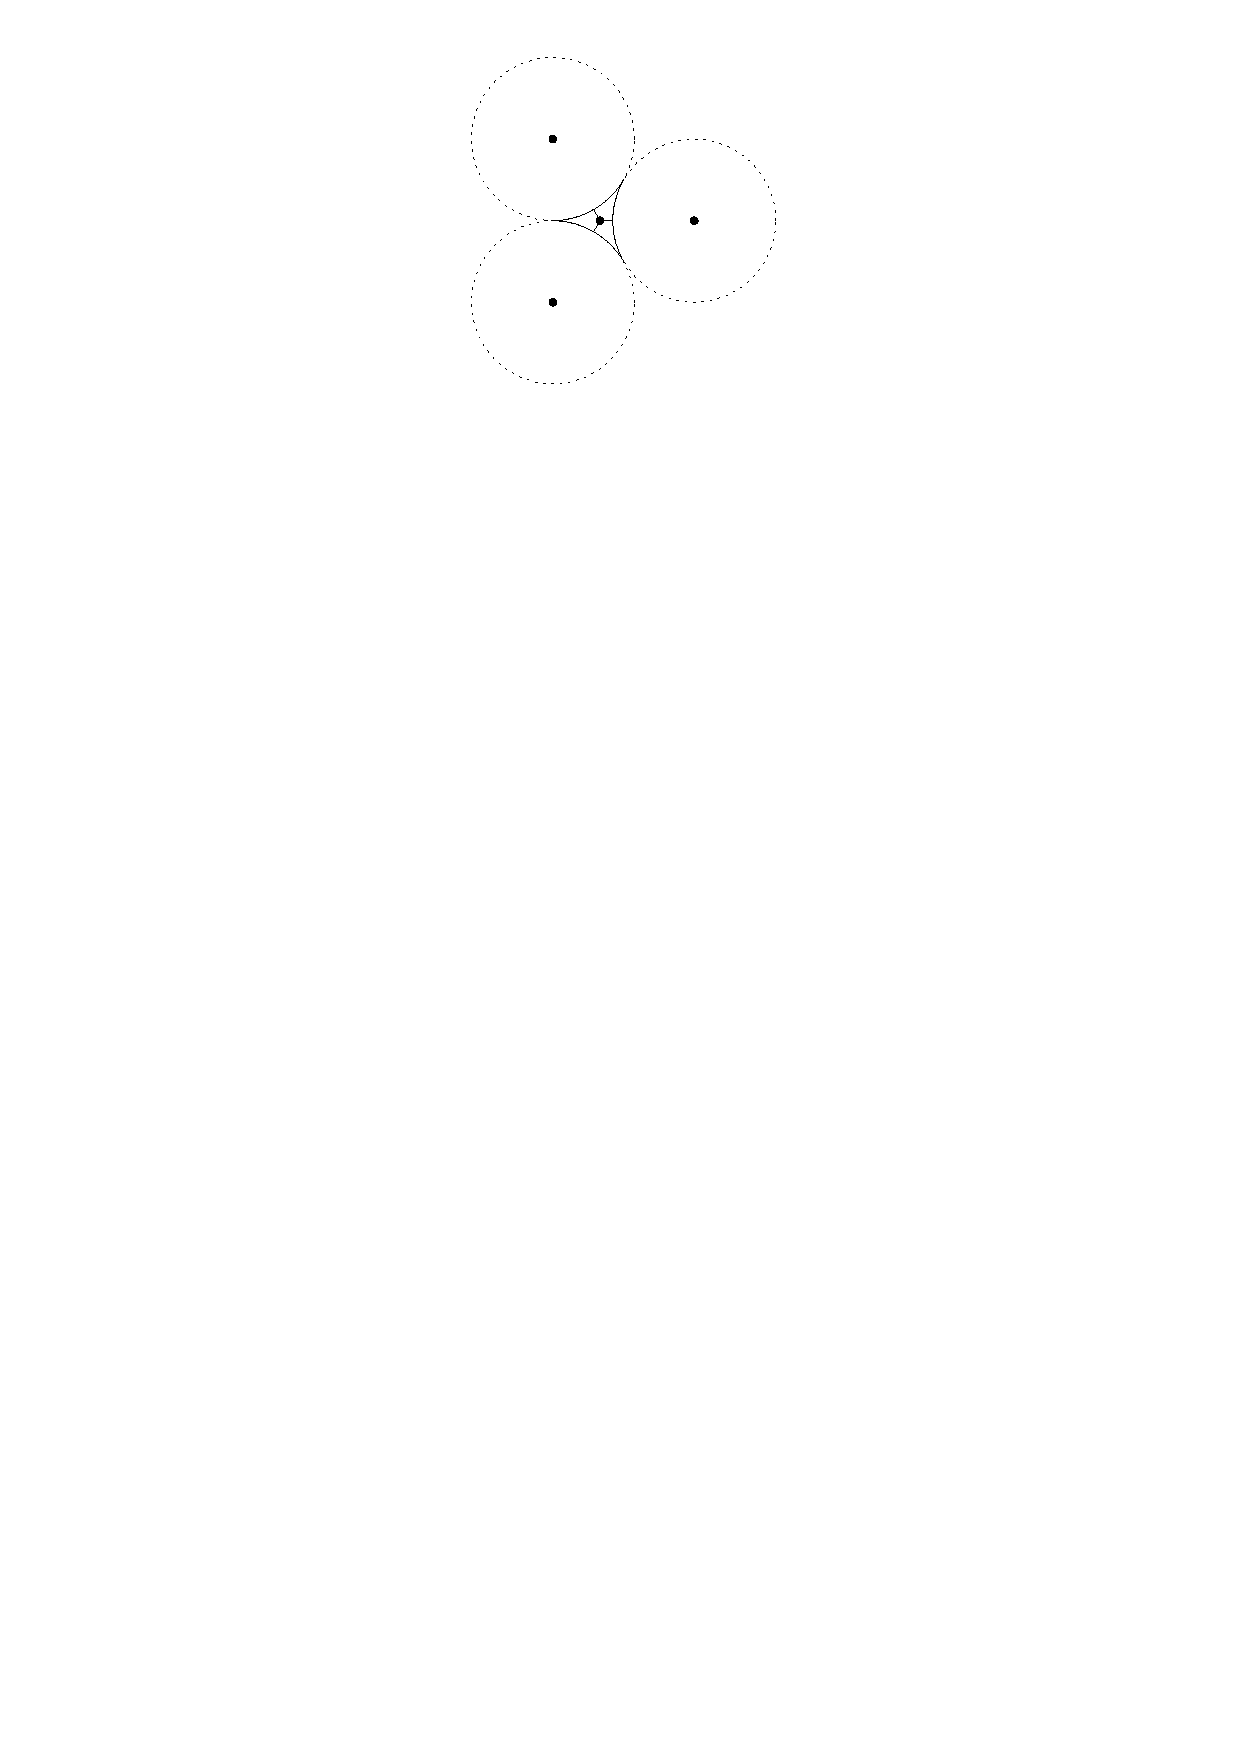
\includegraphics[width=.33\columnwidth]{graphics/dhsi.pdf}
\captionof{figure}{An illustration of the center point in the hexagon $h$ that lies between three adjacent disks of $S_i$.  The distance $d\lr{h,S_i}$ is the length of the line segment from the center point to nearest point of either disk's boundary.}\label{fig:dhsi.pdf}
\end{center}
\end{minipage}

The distance $d\lr{h,S_i} = \frac{\lr{2-\sqrt{3}}r}{\sqrt{3}}$ is from the center point in the hexagon $h$ that lies between three adjacent disks of $S_i$ to the nearest point of either disk's boundary (see Figure \ref{fig:dhsi.pdf}).  
The distance $d\lr{S_i,h} = r$ is the distance from the furthest boundary point of any disk in $S_i$ that lies on the exterior of the hexagon $h$ (see the left illustration in Figure \ref{fig:hexagonPetiolesLeafs9LayersRotatedOutward.pdf}).  
The distance $d\lr{S_i,\sigma_i} \leq \psi_i + 2r$  is the distance from the furthest point on the boundary of an outermost leaf in $\sigma_i$ to the nearest boundary point of $S_i$, a distance of at most $2r$, and the additional coordinate displacement $\psi_i$.  
The distance $d\lr{\sigma_i,S_i}$ is simply the coordinate displacement $\psi_i$.  
We can continue the inequality:
$$\begin{array}{rcl}
H(h,\sigma_i) &\leq&H(h, S_i) + H(S_i, \sigma_i)\\
&=&\text{max} \left\lbrace d\lr{h,S_i}, d\lr{S_i,h} \right\rbrace + \text{max} \left\lbrace d\lr{\sigma_i,S_i}, d\lr{S_i,\sigma_i} \right\rbrace\\
&\leq& \text{max} \left\lbrace \frac{\lr{2-\sqrt{3}}r}{\sqrt{3}}, r \right\rbrace + \text{max} \left\lbrace \psi_i, \psi_i + 2r\right\rbrace\\
&\leq& 3r + \psi_i \\
&=& 3 \frac{\epsilon}{10} + \frac{\zeta(6i-29)}{5 \sqrt{3}}\\
&\leq&\frac{3\epsilon}{10} + \frac{5\epsilon  \sqrt{3}}{2(6i-29)}\frac{\lr{6i-29}}{5 \sqrt{3}}\\
&\leq&\frac{8\epsilon}{10}\\
&\leq&\epsilon
\end{array}
$$

We now show that the number of nodes in $T$ is polynomial in $\epsilon$ and $x$.  
With $i = \ceil{\frac{10x}{\epsilon}}$, the longest path of nodes on a tree from $v_0$ is to the last leaf of any petiole.  This path contains $i$ edges.  The number of nodes in the diameter and including the last leaf of a petiole of $S_i$ corresponding to $T$ is $2(i+1)$.  By squaring the node count of the diameter, we have a generous upper bound of nodes in $T$, $4(i+1)^2$.  This upper bound is a polynomial in $x$ and $\epsilon$ since $i$ is defined as a polynomial in $x$ and $\epsilon$.

\end{proof}

\paragraph{Proof of Theorem \ref{thm:disk}}

\begin{proof}
Given an instance of a P3SAT boolean formula, we can use the snowflake reduction of the modified auxiliary construction.  
Using Lemma \ref{lem:ch4IntroLemma}, we can approximate any hexagon of a given side length with a tree $T$.  
In the modified auxiliary construction in Chapter 3, we had four types of hexagons with different side lengths and the skinny rhombus.  
We can scale the weights (radii) of the corresponding ordered weighted disk contact graph corresponding to $T$ to the rigid frame, obstacle, flag, and half sized hexagons in a modified auxiliary contruction accordingly.  
The rhombus can be approximated by a chain of disks.  
The functionality of the gadgets in the modified auxiliary construction remain the same.

By approximating the polygons in the modified auxiliary construction with the snowflake, we show that Theorem \ref{thm:disk} is a corollary by applying Lemma \ref{lem:ch4IntroLemma}.  
\end{proof}
